% \documentclass{article}

% \usepackage{neurips_2026}
% \usepackage[utf8]{inputenc}
% \usepackage[T1]{fontenc}
% \usepackage{hyperref}
% \usepackage{url}
% \usepackage{booktabs}
% \usepackage{amsfonts}
% \usepackage{nicefrac}
% \usepackage{microtype}
% \usepackage{xcolor}
% \usepackage{graphicx}

% \usepackage{todonotes}
% \setuptodonotes{size=\tiny}

% \title{Grounding Safe-by-Design AI: Can LLMs Construct Formal Situational World Models?}

% \author{%
%   PRISM Fellowship Team \\
%   Working draft for the PRISM team meeting \\
% }

% \begin{document}

% \maketitle

% \begin{abstract}
% Many architectures for Safe-by-design AI systems require explicit models of the situations in which the system
% acts and interacts with humans and other AI systems. Having humans construct such ``situational world models'' does not scale.

% We investigate whether large language models (LLMs) can turn natural-language
% situation descriptions into executable, situational world models encoded in Python. 
% We developed a prompting pipeline in which an LLM generates an implementation of a prescribed abstract base class for partially observed stochastic games, a standard model type used in many learning and planning approaches.
% The implementation is validated, exhaustively rolled out into an explicit
% state--action--transition model, exported as JSON, and analyzed as a
% graph. 
% To evaluate the output, we distinguish interface and rollout validity from semantic correctness.
% Reference fixtures for nine game cases validate the infrastructure, while
% cross-case structural exploratory data analysis characterizes their transition graphs. Preliminary
% experiments with Qwen on the game of Rock--Paper--Scissors show that structurally valid
% generated models can still assign incorrect rewards and player-specific
% observations. These are preliminary results, not a benchmark or a general
% model comparison.
% \end{abstract}

% \section{Introduction}
% \todo{we must agree on an author list and ordering since that is probably part of the online submission form. i suggest alphabetical ordering for simplicity, unless someone vetos this.}
% Formal situational world models are useful in an AI system's decision making when safety-relevant questions
% depend on who can act in a given situation, what actions are available to these stakeholder, and what consequences may
% follow for them with what probabilities, possibly over several steps of interaction. 
% Possible uses of such situational models include computing optimal policies (planning) or assessing possible action plans w.r.t.\ several safety criteria \citep{dalrymple2024guaranteedsafeaiframework}. 
% In some approaches to AI decision making, e.g., those based on metric of human power or empowerment \citep{salge2017empowerment, heitzig2026fair}, it is especially important that not only the possible courses of action of the AI system itself and the likely reactions by humans are represented well, but that in fact the whole range of possible human behaviors is covered, if only in rough approximation. 

% This project's aim is to determine whether LLMs can construct simple forms of such
% models from ordinary-language situation descriptions, rather than requiring
% each model to be human-authored or learned. 

% The presentation that motivated this work
% emphasized eventual analyses of agent and human options; the current paper does
% not claim to measure power or empowerment. Instead, it reports the implemented
% pipeline for constructing and inspecting executable situational models.

% Our current question is deliberately narrower: after an LLM generates a Python
% world model, can we validate, roll out, and characterize the resulting model
% without asking the LLM to provide a second declarative representation? The
% Python track answers this operational question by treating the generated Python
% program as the world model and deriving an explicit representation from its
% transition interface.

% \section{Related Work}

% % TODO: Add a literature review and citations covering stochastic games,
% % partially observable models, LLM program generation, and world-model
% % evaluation before submission.
% This working draft does not yet include a completed literature review. The
% present contribution is therefore methodological and empirical in scope: a
% small executable-model pipeline and preliminary observations from its use.

% \section{Proposed Method}

% \subsection{Preliminaries}

% We use a lightweight, stateless \texttt{AbstractPOSG} interface. A generated
% model exposes explicit player identifiers, legal actions, an initial state,
% transition distributions, observations, rewards, and terminal-state detection.
% Joint actions are dictionaries keyed by player identifiers. States must be
% hashable so that the reachable model can be enumerated. The abstraction is
% intentionally compact enough for an LLM to implement while retaining the
% dynamics needed for multi-agent analysis.

% The generated Python object is the world model. A PettingZoo
% \texttt{ParallelEnv} adapter is retained as an execution-compatibility layer
% for multiplayer environments, but it is not the world-model representation
% used for the analyses below.

% \subsection{World-Model Generation and Rollout}

% Given a natural-language situation, a local Ollama/Qwen setup generates a
% \texttt{GeneratedPOSG(AbstractPOSG)} class. The generation prompt requires
% executable Python, explicit players and joint actions, hashable state
% identifiers, and valid finite transition probabilities. It does not guarantee
% semantic correctness.

% Generated code is executed before rollout. The pipeline records failures such
% as execution errors, unhashable initial states, malformed actions or
% transitions, invalid probabilities, and invalid terminal structure; it does
% not silently repair generated code. For a valid finite model, exhaustive
% rollout explores reachable non-terminal states up to configurable state and
% depth limits. At each state it enumerates legal joint actions, records
% successor distributions, and retains observations and rewards. The result is
% an explicit reachable world model containing players, initial distribution,
% states, terminal states, action sets, joint actions, transitions, probabilities,
% observations, and rewards.

% Canonical JSON is exported \emph{after} this rollout. Thus, in the Python
% track, JSON is algorithmically derived from the executable Python model rather
% than generated by the LLM.

% \subsection{Evaluation and Structural Analysis}

% The explicit rollout supports two graph representations: a directed
% state-transition graph and a state--action--transition graph that preserves
% joint-action labels and transition probabilities. We use graph quantities such
% as reachable and terminal state counts, edge counts, branching, deterministic
% and stochastic transition fractions, transition entropy, depth, strongly
% connected components, centrality, efficiency, and action influence as
% exploratory data analysis (EDA). They are structural descriptors of generated
% world-model graphs, not established measures of LLM world-model quality.

% The project test cases provide natural-language inputs, expected outputs where
% the setting is sufficiently closed, and include/must-not judging criteria.
% They cover toy, game, situational, and cultural-norm settings. For the Python
% track, executable G1--G9 reference-schema fixtures are control cases: they
% exercise rollout, canonical export, graphs, and EDA, but are not LLM-generated
% results.

% \section{Results and Discussion}

% \subsection{Infrastructure Controls and Cross-Test-Case Structural EDA}

% The G1--G9 executable reference fixtures successfully exercise the current
% Python rollout, canonical export, graph construction, and EDA pipeline. These
% are infrastructure controls rather than LLM outputs. Table~\ref{tab:fixture-eda}
% reports the cross-case measurements from the generated EDA report. They cover
% deterministic and stochastic transitions, different branching factors, and both
% one-step and multi-step structures. G6 is the only multi-step fixture; it has
% maximum depth two and an average terminal distance of 1.29, whereas all other
% fixtures have maximum depth one and average terminal distance one.

% \begin{table*}[t]
% \centering
% \caption{Cross-test-case structural EDA for executable G1--G9 reference
% fixtures. These are control schemas used to validate the pipeline, not
% LLM-generated performance results. Entropy is measured in bits; average path
% is average terminal distance.}
% \label{tab:fixture-eda}
% \small
% \setlength{\tabcolsep}{3pt}
% \begin{tabular}{lrrrrrrrrr}
% \toprule
% Case & States & Terminal & Joint actions & Avg.\ branch & Stoch.\ \% &
% Avg.\ entropy & Max depth & SCCs & Avg.\ path \\
% \midrule
% G1 & 4 & 3 & 9  & 2.25 & 0   & 0.000 & 1 & 4 & 1.00 \\
% G2 & 4 & 3 & 1  & 0.25 & 100 & 1.483 & 1 & 4 & 1.00 \\
% G3 & 4 & 3 & 4  & 1.00 & 50  & 0.500 & 1 & 4 & 1.00 \\
% G4 & 3 & 2 & 9  & 3.00 & 0   & 0.000 & 1 & 3 & 1.00 \\
% G5 & 3 & 2 & 4  & 1.33 & 0   & 0.000 & 1 & 3 & 1.00 \\
% G6 & 6 & 4 & 5  & 0.83 & 20  & 0.200 & 2 & 6 & 1.29 \\
% G7 & 5 & 4 & 4  & 0.80 & 0   & 0.000 & 1 & 5 & 1.00 \\
% G8 & 5 & 4 & 4  & 0.80 & 0   & 0.000 & 1 & 5 & 1.00 \\
% G9 & 5 & 4 & 16 & 3.20 & 0   & 0.000 & 1 & 5 & 1.00 \\
% \bottomrule
% \end{tabular}
% \end{table*}

% \begin{figure}[t]
% \centering
% 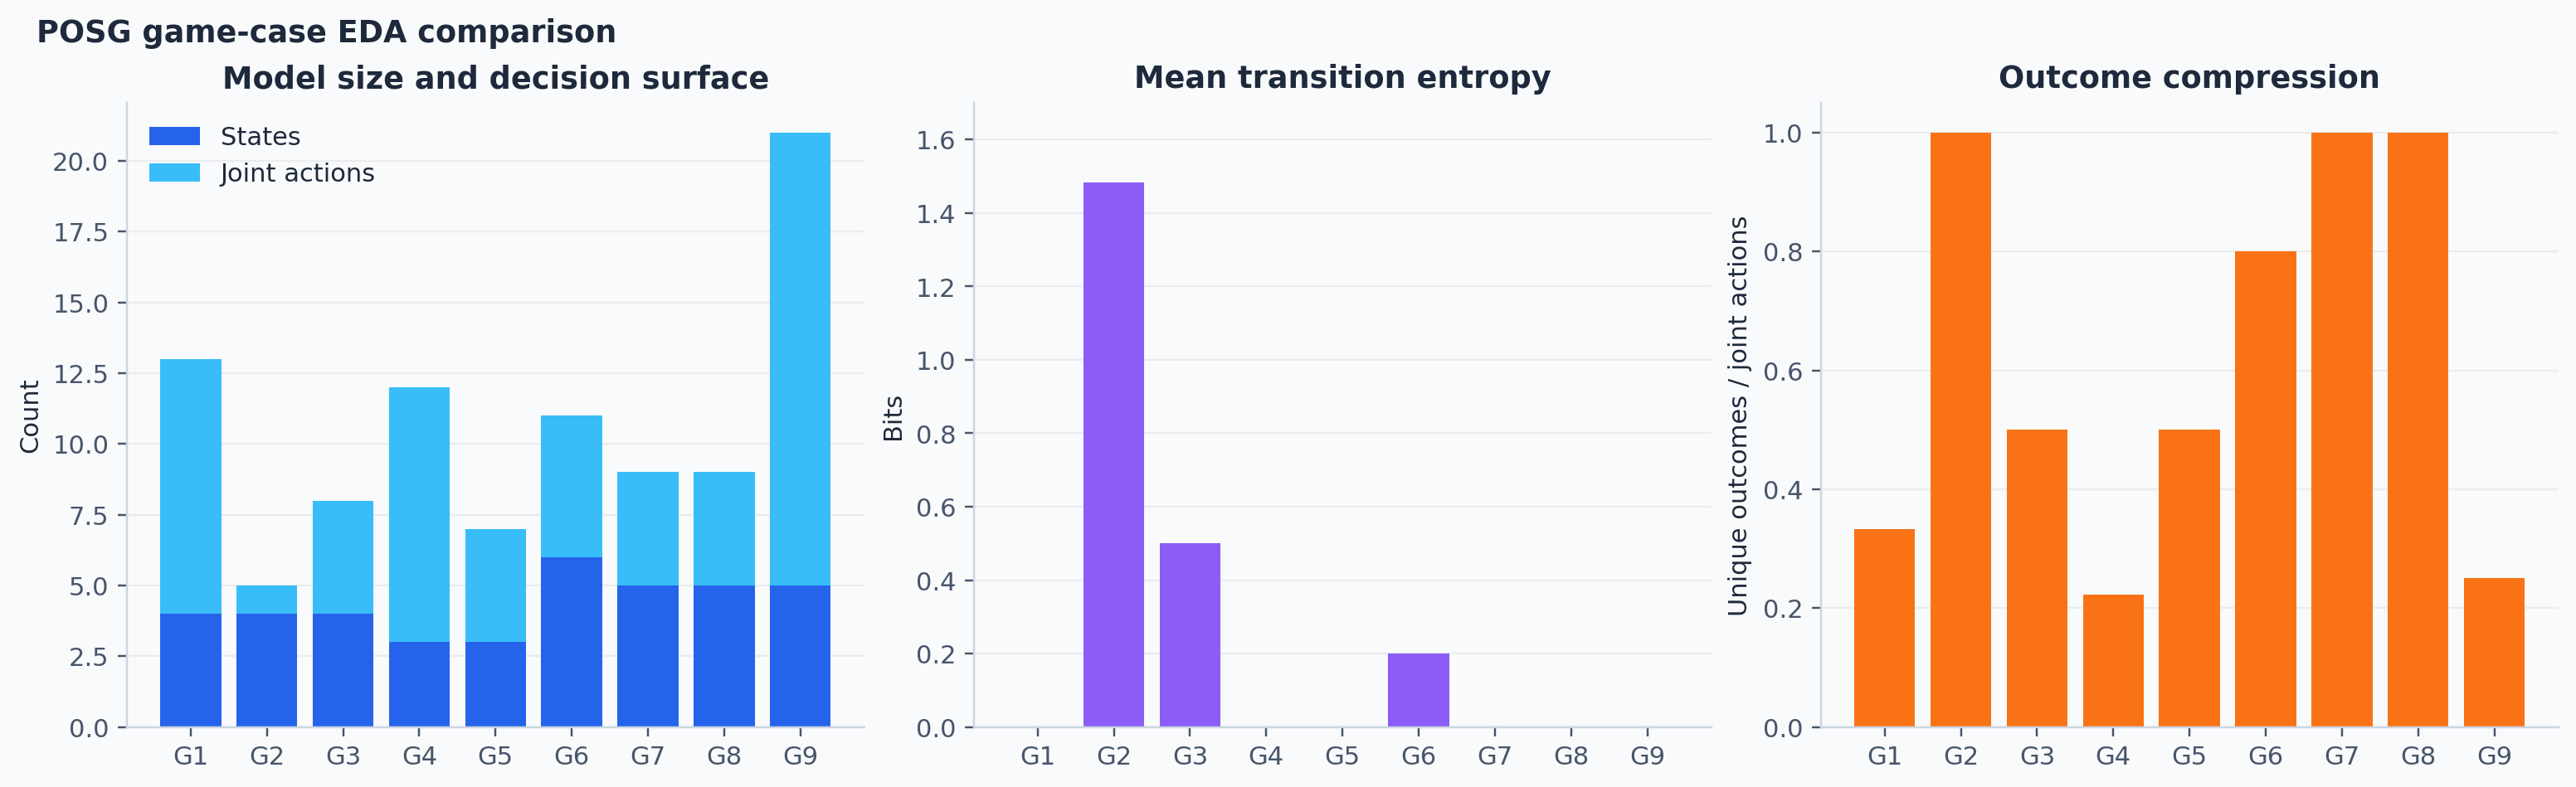
\includegraphics[width=\linewidth]{figures/game_case_comparison.png}
% \caption{Cross-case comparison generated from the G1--G9 reference fixtures.
% The figure makes the variation in declared state/action structure and
% transition properties visible before applying the same analysis to generated
% models. It is an infrastructure-characterization figure, not an LLM ranking.}
% \label{fig:fixture-comparison}
% \end{figure}

% The reference EDA confirms that the analysis is not restricted to the
% deterministic Rock--Paper--Scissors control: G2 is entirely stochastic, G3 is
% half stochastic, and G6 includes a longer reachable trajectory. The state
% graphs have between three and six strongly connected components in this small
% fixture set. These measurements describe the declared schemas and provide
% known structural variation against which rollout and graph extraction can be
% checked.

% \subsection{Generation and Execution Results}

% Table~\ref{tab:generation-results} separates three different evidence sources.
% The 12-task GridWorld experiment is a small pre-existing Codex-generated
% Python harness pilot: its 72/72 probe checks passed, but its worlds are
% templated GridWorld programs rather than POSGs, so it is retained only as an
% implementation sanity check. The G1--G9 controls above establish POSG
% infrastructure behavior. The Qwen artifacts are the current LLM-generated
% POSG evidence and are evaluated separately below.

% \begin{table}[t]
% \centering
% \caption{Recorded generation and execution evidence. Rates in the GridWorld
% pilot are not treated as general world-model performance metrics.}
% \label{tab:generation-results}
% \small
% \begin{tabular}{p{0.30\linewidth}p{0.17\linewidth}p{0.43\linewidth}}
% \toprule
% Source & Scope & Recorded outcome \\
% \midrule
% Codex GridWorld pilot & 12 tasks & 72/72 probe checks passed; execution,
% behavioral, answer, and simulator-fidelity rates reported as 1.0 \\
% G1--G9 POSG fixtures & 9 controls & Rollout and EDA completed for declared
% reference schemas \\
% Qwen G1, samples 003--008 & 6 generated POSGs & All completed structural
% pipeline; semantic checks failed \\
% Qwen failures & 4 retained artifacts & G1: unhashable state and prompt-format
% failure; G9: unhashable state and invalid transition \\
% \bottomrule
% \end{tabular}
% \end{table}

% \subsection{Preliminary Qwen Experiments}

% The experiment runner records generation, execution, validation, rollout,
% graph-construction, EDA, and total time, together with optional Python-level
% memory allocation and generated artifacts. In an initial Qwen pilot, generation
% time dominated the small-case runtime, but the first G1 and G9 generations
% failed validation. Their generated source and failure records were retained.

% After a prompt revision that included a minimal valid interface skeleton and
% explicit hashable-state guidance, Qwen G1 samples 003--008 completed the
% structural pipeline. Each had four reachable states, three terminal states,
% nine joint actions, deterministic one-step transitions, three collapsed
% state-transition edges, zero average transition entropy, maximum depth one,
% and four strongly connected components. Generation took 11.66--18.89 seconds
% per successful sample; total recorded time was 11.67--18.90 seconds. The
% remaining pipeline stages were correspondingly small for these tiny models.

% \begin{figure}[t]
% \centering
% 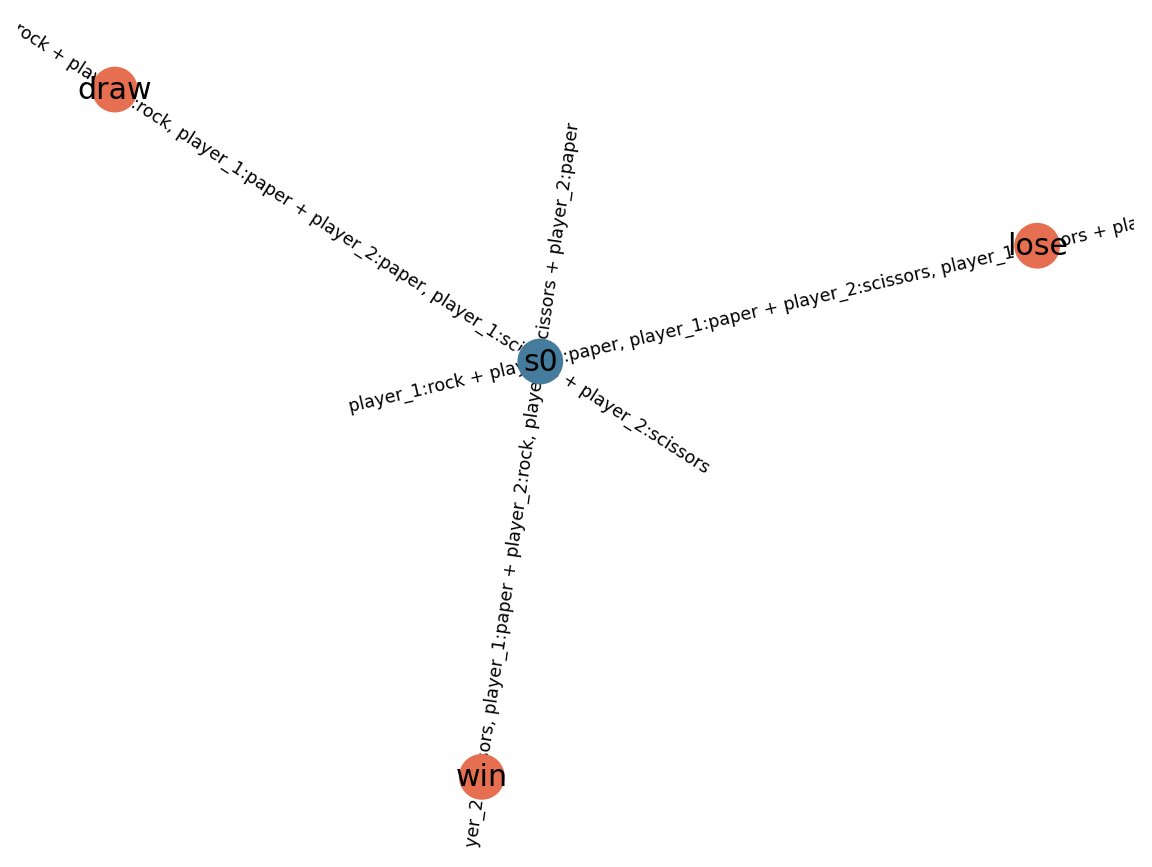
\includegraphics[width=\linewidth]{figures/qwen_g1_sample_003_graph.png}
% \caption{State graph exported from Qwen G1 sample 003 after validation and
% exhaustive rollout. Samples 003--008 share this same structural profile. The
% semantic result in Table~\ref{tab:g1-semantics} shows why this apparently
% well-formed graph is insufficient evidence of a correct game model.}
% \label{fig:qwen-g1-graph}
% \end{figure}

% The two retained G9 attempts illustrate distinct failure modes. Sample 001
% used an unhashable initial state. Sample 002 reached transition execution but
% failed when generated code compared allocation strings such as
% \texttt{"0+3"} directly with integers. These outcomes are recorded rather than
% repaired, so the artifacts retain evidence of where generation or execution
% failed.

% \subsection{G1 Semantic Inspection}

% We added a small, explicit semantic oracle for the single-round
% Rock--Paper--Scissors case. It checks the two expected players, action sets,
% simultaneous coverage of all nine joint actions, deterministic transition
% partitioning, conventional zero-sum rewards, three terminal outcome states,
% and lightweight consistency of player-specific observations. Each check returns
% \textsc{pass}, \textsc{fail}, or \textsc{unknown}. The optional semantic score
% is only the fraction of applicable checks that pass; it is not a validated
% research metric.

% For all six successful Qwen G1 samples, structural validity and transition
% partitioning passed, while reward and observation checks failed. In particular,
% the generated models could partition actions into win/lose/draw outcomes while
% assigning both players a loss reward in a losing outcome or reporting that the
% wrong player won. This is a preliminary observation from six samples of one
% model and one game, but it demonstrates why structural validity, rollout
% validity, semantic correctness, and graph EDA must remain separate.

% \begin{table}[t]
% \centering
% \caption{G1 semantic-oracle results for the six structurally successful Qwen
% samples. The oracle is specific to the G1 Rock--Paper--Scissors setting.}
% \label{tab:g1-semantics}
% \small
% \begin{tabular}{lccccc}
% \toprule
% Samples & Structural & Transition & Reward & Observation & Semantic score \\
% \midrule
% 003--008 (6) & PASS & PASS & FAIL & FAIL & 0.75 \\
% \bottomrule
% \end{tabular}
% \end{table}

% Table~\ref{tab:g1-semantics} makes the central distinction explicit:
% structural and rollout success do not imply semantic correctness. The
% state/action graph in Figure~\ref{fig:qwen-g1-graph} is therefore useful for
% exploratory structural characterization, but not a substitute for a
% situation-specific correctness check.

% \subsection{Limitations}

% The current number of real LLM experiments is small and Qwen-focused. The G1
% semantic oracle is a concrete correctness mechanism for one closed game, not a
% general semantic evaluator. Reference fixtures are infrastructure controls,
% not LLM results. Exhaustive rollout is bounded by configured state and depth
% limits, and structural graph similarity does not guarantee correct rewards,
% observations, or dynamics. The GridWorld pilot lacks the representation and
% independent raw-generation evidence needed for comparison with the POSG track.
% % TODO: Add multi-model POSG comparison after GLM/Kimi experiments.

% \section{Conclusion}

% The current Python track provides an executable route from a natural-language
% situation description to a generated situational world model, more specifically a partially observed stochastic game encoded as a python class deriving from a prescribed abstract base class. This can then be used to query transition probabilities in order to roll out a full list of players, states, actions, and transitions. The latter can be exported into a flat JSON data structure that represents the situational world model in an explicit way and complies to a suitable schema. Our code-base also provides abilities for graph representations and exploratory structural analysis. Preliminary
% results from experiments with Qwen \todo{what model exactly?} show that this pipeline can produce structurally valid, small situational
% world models while still exposing semantic errors that graph structure alone
% does not reveal. The next step is controlled expansion to additional cases and
% models, paired with carefully scoped semantic checks rather than conflating
% structural validity with correctness.

% \section{References}

% % TODO: Add references when the related-work section is completed.

% \end{document}